\chapter{Importance sampling}

\section{Comparison of importance sampling to the \enquote{crude} method}%
\label{ex:031}

\begin{sourcefiles}
  \item[Source codes] src/031\_crude\_vs\_importance.c
  \item[Analysis scripts] src/031\_crude\_vs\_importance.R
  \item[Executables] exe/031\_crude\_vs\_importance
\end{sourcefiles}

The goal was to integrate the function $f(x) = g(x) e^{-x^{2}}$ on $[0,
\infty)$, with $g(x)$ being a slowly varying function. I chose $g(x) = x
\cos x^{2}$, so the exact value of the integral is
\begin{equation}
  \int_{0}^{\infty} f(x) \, dx = \int_{0}^{\infty} x \cos(x^2) e^{-x^{2}}\, dx =
  \dots = \frac{1}{4}.
\end{equation}
Following the suggestion, we multiply and divide by a weighting function defined
as
\begin{equation}
  w(x) = \frac{2}{\sqrt{\pi}} e^{-x^{2}},
\end{equation}
and so we can write
\begin{equation}
  \int_{0}^{\infty} g(x) e^{-x^{2}} \, dx = \frac{\sqrt{\pi}}{2}
  \int_{0}^{\infty} g(x) w(x) \, dx = \frac{\sqrt{\pi}}{2} \int_{0}^{\infty}
  g(x) \, dw(x).
\end{equation}
Therefore, we can sample numbers $x_i$ from $w(x)$ and estimate the integral
with
\begin{equation}
  \int_{0}^{\infty} g(x) e^{-x^{2}} \, dx \approx \frac{\sqrt{\pi}}{2N} \sum_{i
  = 1}^{N} g(x_i).
\end{equation}

To sample from $w(x)$, which is a half-normal distribution with variance $1/2$,
we can use a modified Box-Muller. The idea is to restrict the number generation
to the $x > 0$ half-plane. First, since in this case the variance is not
unitary, we can recompute the cumulative. The marginal distribution over $r$
needs a factor \num{2} in front for normalization, and we obtain
\begin{equation}
  \rho_r(r) = 2re^{-r^{2}} \implies F_r(r) = 1 - e^{-r^{2}} \implies r =
  \sqrt{-\log(1 - u_{1})}, \quad\text{with } u_1 \sim \unif{0}{1}.
\end{equation}
For $\theta$ we sample uniformly over $[-\pi/2, +\pi/2]$ in order to stay in the
$x > 0$ half-plane:
\begin{equation}
  \theta = -\frac{\pi}{2} + \pi u_2, \quad \text{with } u_2 \sim \unif{0}{1}.
\end{equation}
Once we have $r$ and $\theta$ we generate $x$, $y$ distributed according to
$w(x)$ in this way:
\begin{equation}
  x = r \cos\theta,\quad y = r\abs{\sin\theta}.
\end{equation}

In contrast to the importance sampling technique, inside the same C file I also
implemented the \enquote{crude} Monte Carlo integration, that is a simple
average of a set of $f(x_i)$ with $x_i$ sampled uniformly over an interval from
$0$ to a given $x_{\mathrm{max}}$:
\begin{equation}
  \int_{0}^{\infty} g(x) e^{-x^{2}}\, dx \approx \frac{1}{N} \sum_{i = 1}^{N}
  g(x_i) e^{-x_i^2}, \quad \text{with } x_i \sim \unif{0}{x_{\mathrm{max}}}.
\end{equation}
You can see the comparison between the two methods in terms of relative error in
\figref{fig:031}. The importance sampling is definitely more efficient, although
the crude method has a higher variance which can lead to a lower error in lucky
runs. Also, as the number of samples grows the difference between the two
methods shrinks, but this is rather unsurprising.

\begin{figure}
  \centering
  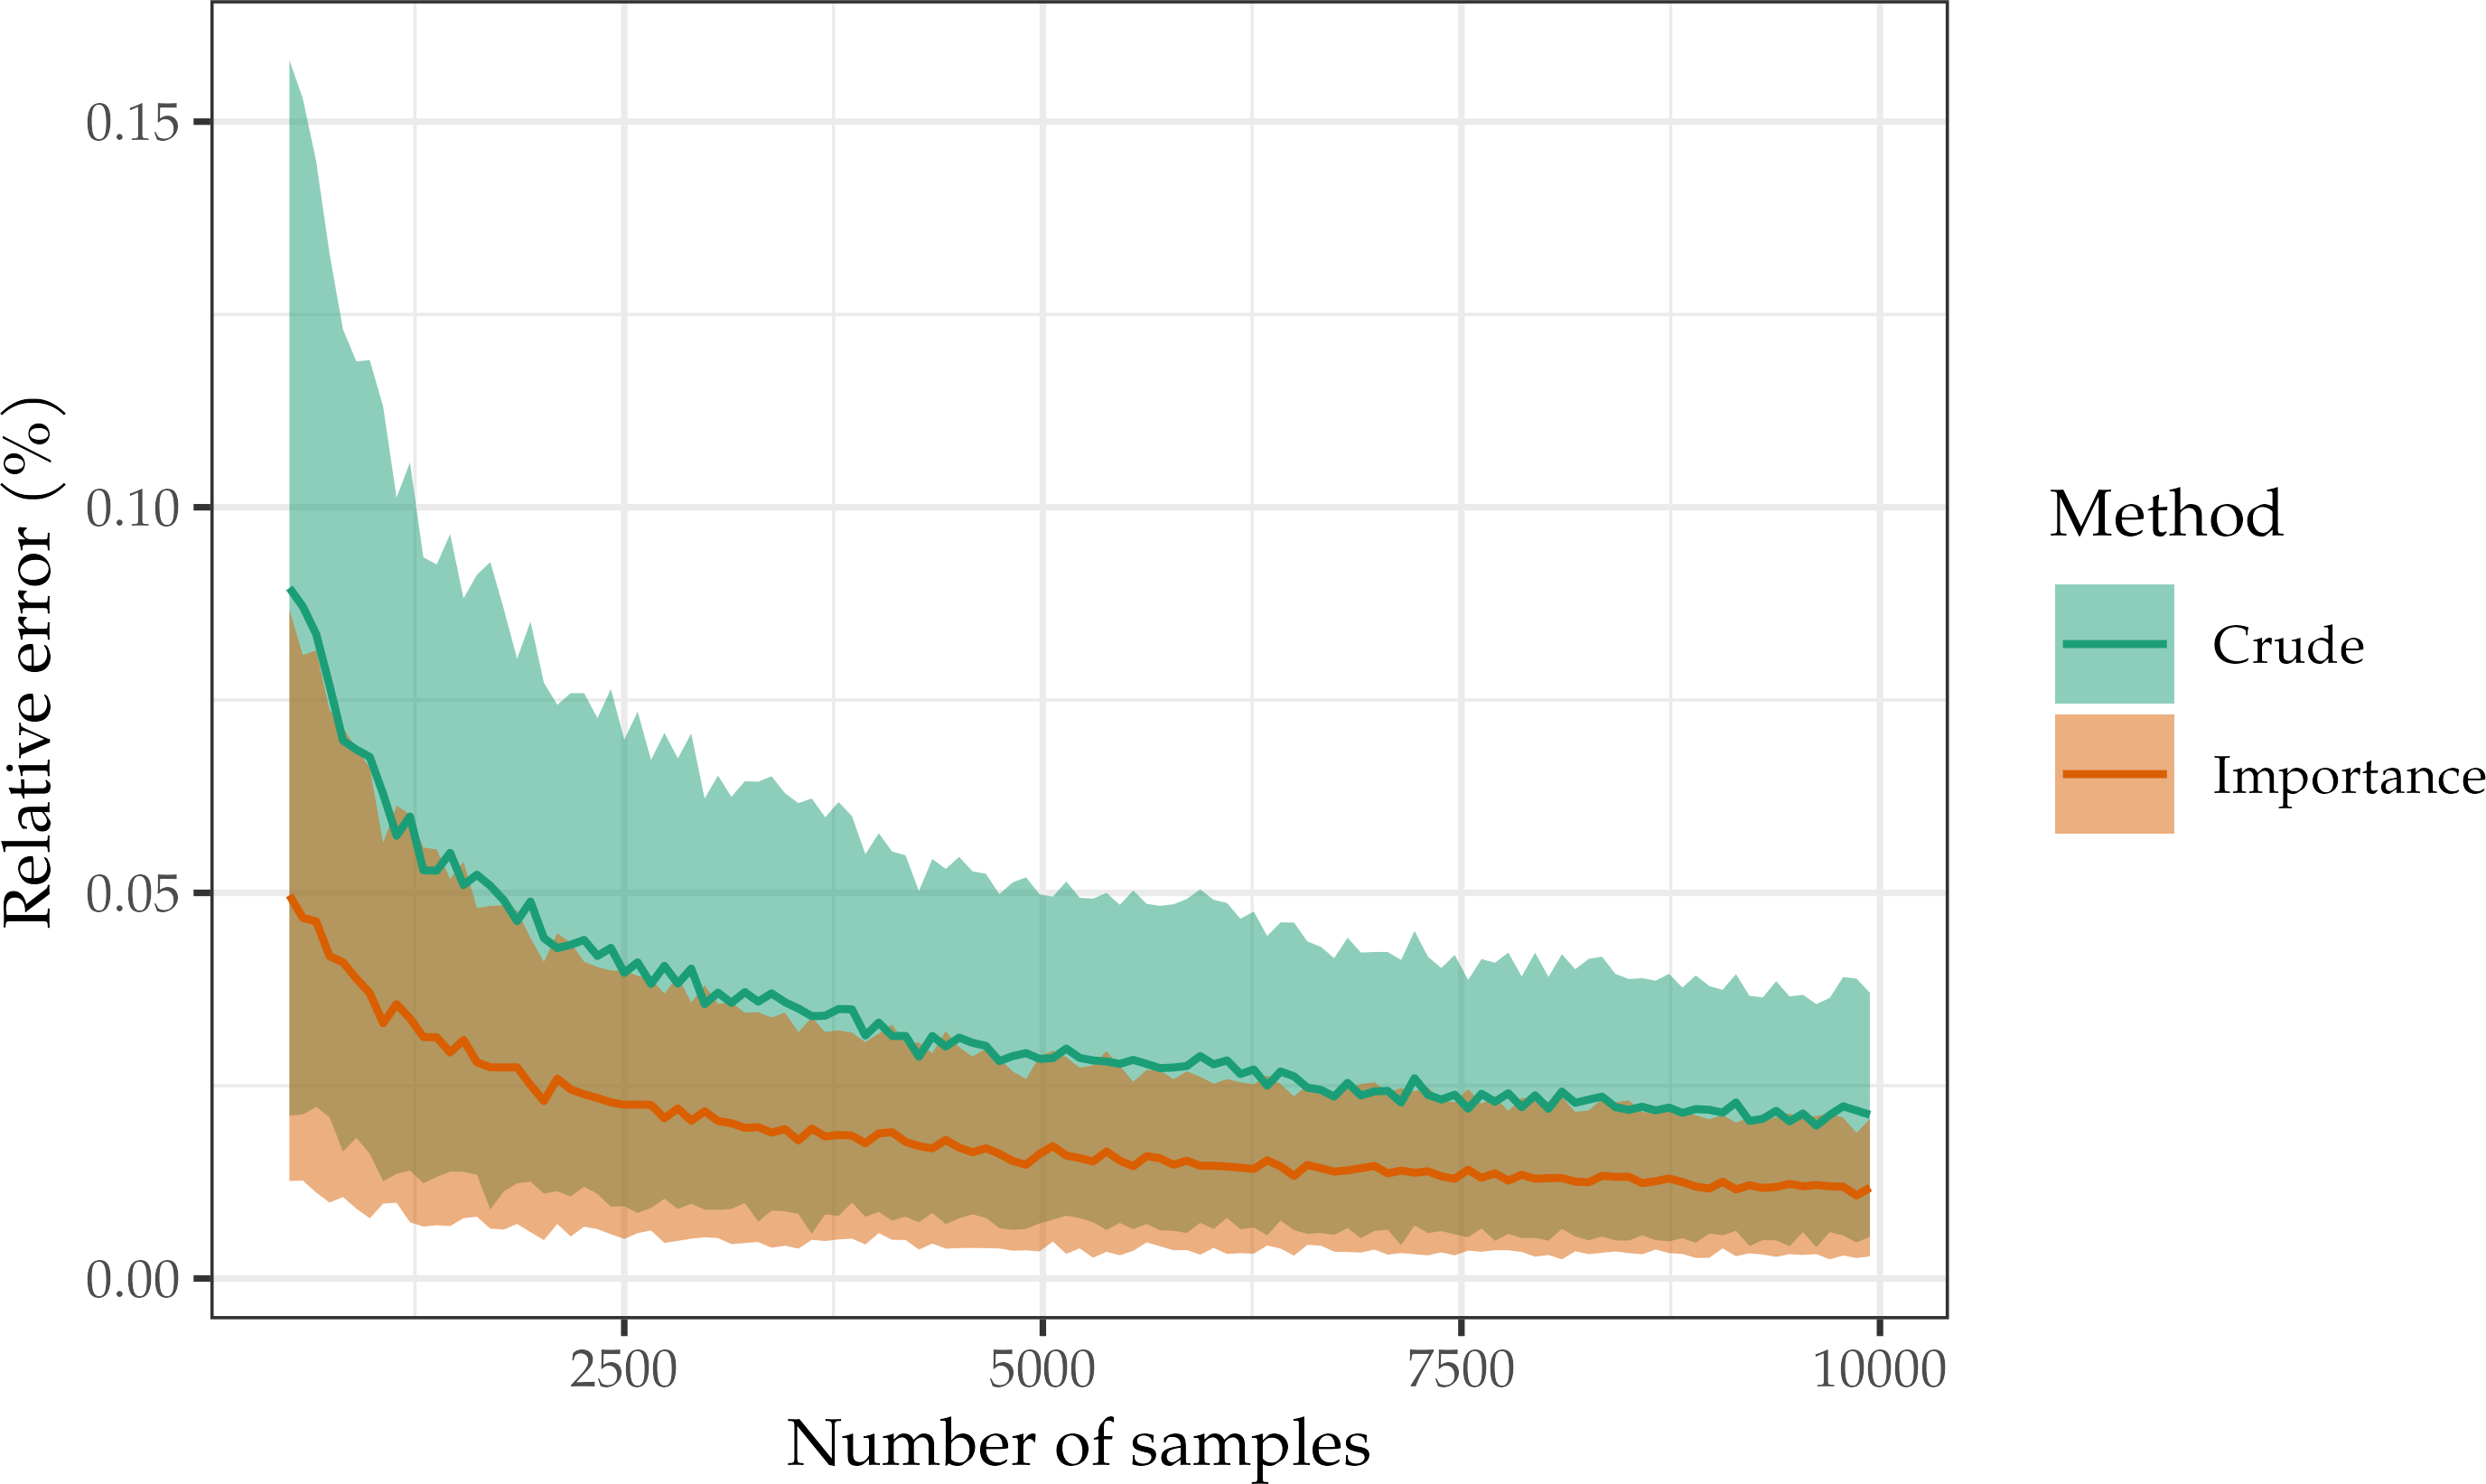
\includegraphics{img/031.png}
  \caption{comparison of the relative error between a \enquote{crude} Monte
    Carlo integration and importance sampling as a function of the number of
    samples. The solid lines represent the average over \num{100} realizations,
    with the standard deviation shaded in the same colour.}
  \label{fig:031}
\end{figure}
